% Manual for circbuf
% Copyright (c) 2007 Lennart Yseboodt

\documentclass[a4paper]{article}

\usepackage{graphicx}
\usepackage{listings}

\begin{document}

	\title{CircBuf 1.0}
	\author{Lennart Yseboodt}
	\date{\today}

	\maketitle

	\tableofcontents

	\lstset{language=C,basicstyle=\small}

\setlength{\parindent}{0pt}
\setlength{\parskip}{1ex minus 0.2ex plus 0.5ex}
	
\section{Introduction}
This manual describes the operation of CircBuf, a compact implementation of circular buffers.
This circular buffer acts as a FIFO (First In First Out). They are thread-safe and deadlock free.

FIFO's are commonly used to communicate between two separate control flows in a microprocessor.
This can be between two processes running under a scheduler, or in a system without an operating system
to communicate between interrupt routines and the main routine of the program.

Circbuf allows you to put data elements in a fifo and later retrieve them. You choose yourself how large
a single data element is and how many of them there are. You are responsible for allocating the memory
and passing the pointer to the initialization routine.

To use the fifo you make a request to read or a request to write. You get a pointer back that is zero if
there is no data available or no space available respectively. If you get a valid pointer you can read or
write from it. You must ensure not to write or read to much, there is no memory protection.

\begin{figure}
	\centering
	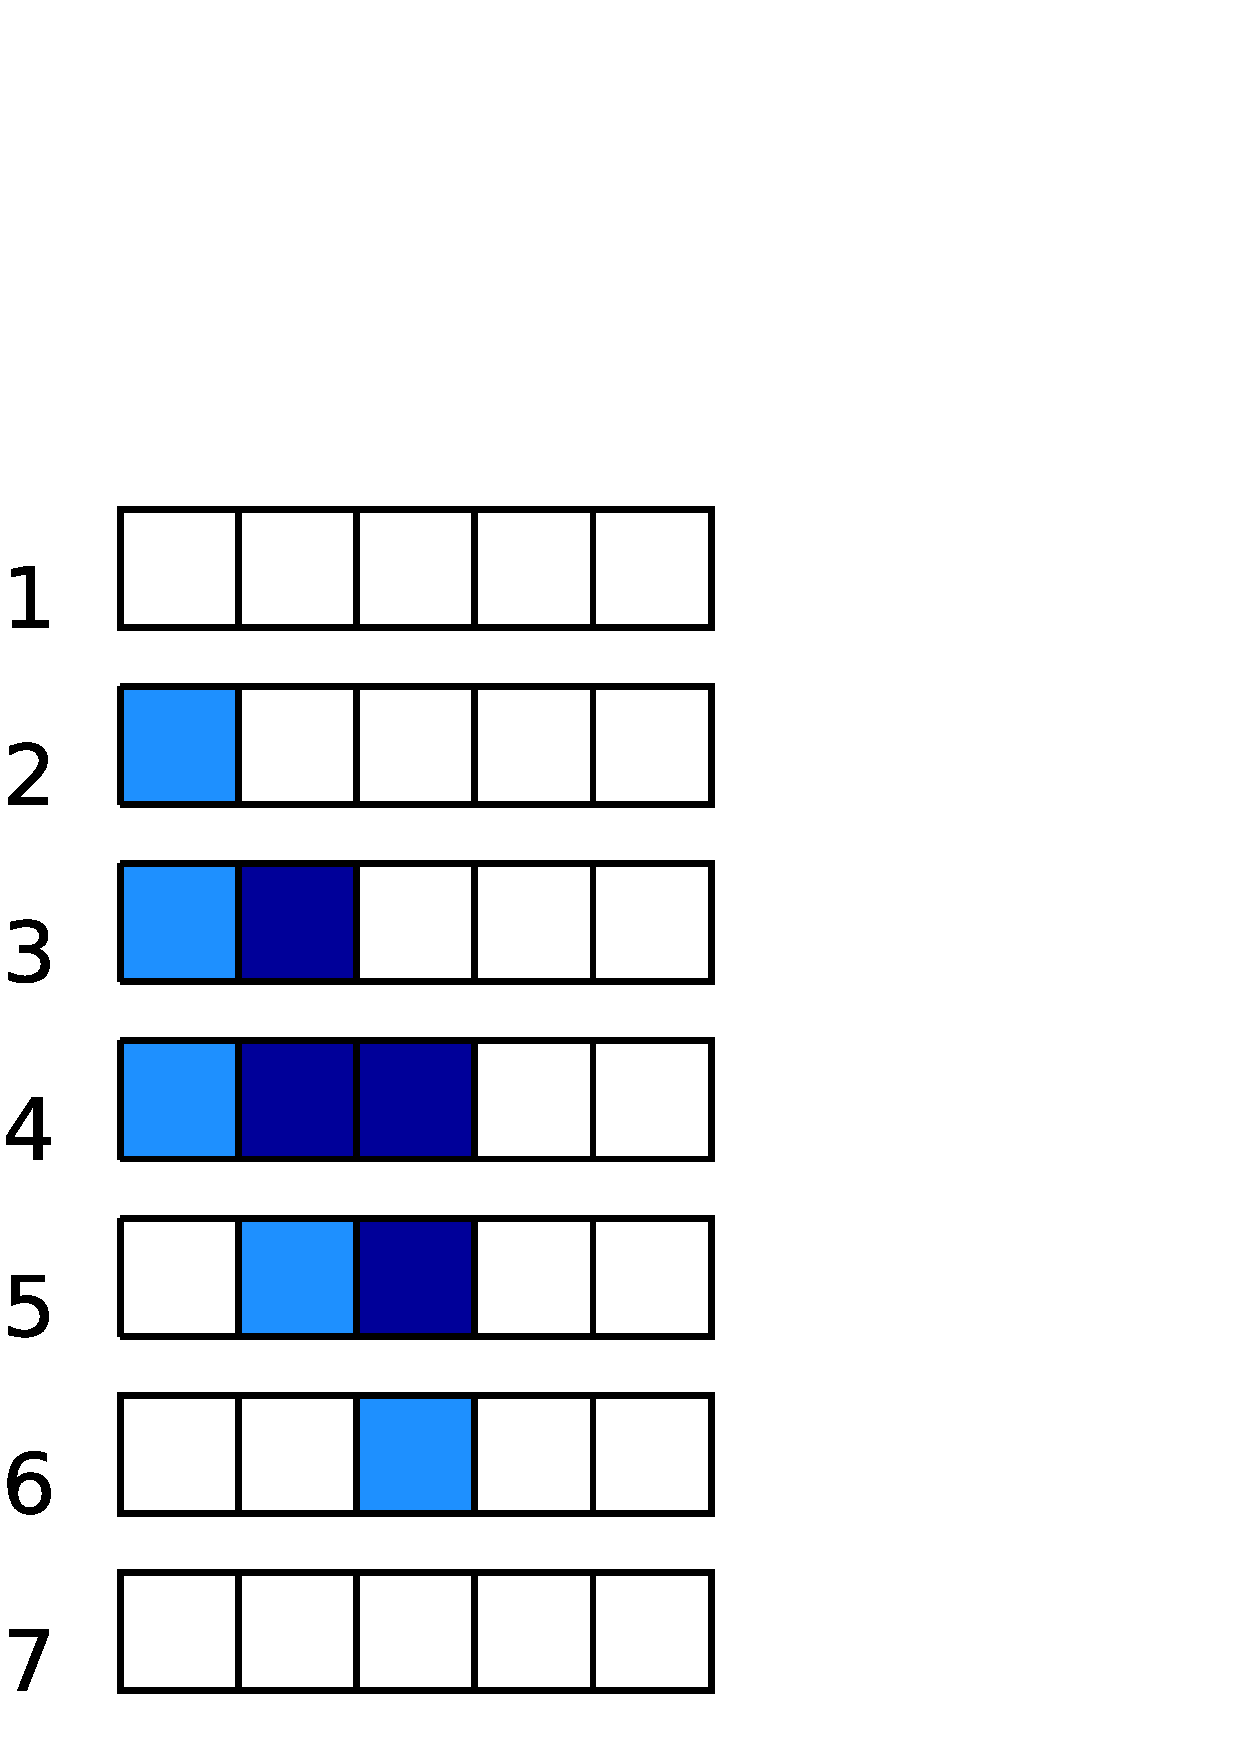
\includegraphics[width=.4\textwidth]{diagrams/fifo.pdf}
	\caption{Basic FIFO operation. Light blue is the element that was added last and will be read first}
	\label{fig:fifo}
\end{figure}

\subsection{FIFO's}
An example session with a FIFO is shown in Figure \ref{fig:fifo}. A white block means that element is empty.
Blue means it is filled with data. The light blue element is the element that was last written to the FIFO.
The light blue element is also the one you will get when you make a read request. First element in, first element out.

The example starts with all 5 elements empty (white). This is step 1.
In step 2 an element is written. In step 3 and 4 two more elements are written.
Three places are no filled, the light blue one is the one that was written first.
In step 5 a read request is made and the light blue element is read.
Now the next element becomes light blue (next to read). In step 6 and 7 the element are read out.
Step 7 leaves the FIFO empty.

\subsection{Getting started}
In the \texttt{app} directory are some simple examples that you can take a look at.
There is a very simple example and one with threads. For the one with threads you need the
pthread and ncurses library, so it will probably only work on unix systems.
The other one should work on Windows as well. Now, how to get started ?
Say we want a FIFO with 4 byte elements, and we want to have room for 10 of them.

\begin{enumerate}
	\item We allocate 40 bytes. \lstinline!char buffer[40];! or, if you have malloc, \lstinline!char *buffer=malloc(40);!
	\item Next we need the object that represents our FIFO. We declare \lstinline!CircularBuffer cb;!
	\item The CircularBuffer object must be initialized with the \texttt{cb\_init()} function.
	      So you call \lstinline!cb_init(&cb,buffer,10,4);! The first argument is always a pointer to cb. For the init function
	      the second argument is a pointer to the buffer memory. The third argument is the number of elements your FIFO is deep.
	      The last argument is how large (in bytes) each element is.
	\item Now we can use our CircularBuffer. We will put the number 0, 1 and 2 in it.
		\begin{lstlisting}
int *d;

d = cb_writePacket(&cb); /* Get buffer */
*d = 0; /* Write buffer */
cb_doneWritePacket(&cb); /* Don't forget to confirm you are done! */

d = cb_writePacket(&cb); /* Get buffer */
*d = 1; /* Write buffer */
cb_doneWritePacket(&cb); /* Don't forget to confirm you are done! */

d = cb_writePacket(&cb); /* Get buffer */
*d = 2; /* Write buffer */
cb_doneWritePacket(&cb); /* Don't forget to confirm you are done! */
		\end{lstlisting}
	\item We can now read out these values again and print them on screen.
		\begin{lstlisting}
int *d,c;

for(c=1;c<=3;c++){
	d = cb_readPacket(&cb); /* Get buffer */
	printf("%d\n",*d); /* Print value */
	cb_doneReadPacket(&cb); /* Confirm done */
}
		\end{lstlisting}
\end{enumerate}

You can find this complete example in the \texttt{app} directory under the file \texttt{numbers.c}.

\section{Compiling CircBuf}
There is only one source file, called \texttt{circbuf.c} that includes two header files (\texttt{circbuf.h, types.h}).
If your project uses a Makefile you need to add this file in the appropriate place, if you have a graphical environment
you can simply add it to your project. This library depends on no other libraries, not even the standard C library.

\section{Reference}

\subsection*{\texttt{cb\_init()}}
Syntax: \lstinline!void cb_init(CircularBuffer *cb, euint8* mem, euint32 numsectors, euint32 sectorsize);!

This function must be called before a CircularBuffer object can be used. The first argument (cb) is a pointer to
the CircularBuffer object. The second argument (mem) is a pointer to the FIFO memory. This must be allocated by the caller of
\texttt{cb\_init()}. The third argument (numsectors) is the number of slots in the FIFO, and finally the last argument is the
size of each slot (sectorsize).

There is no return value.

\subsection*{\texttt{cb\_readPacket()}}
Syntax: \lstinline!euint8* cb_readPacket(CircularBuffer *cb);!

This function is used to retrieve an element from the FIFO. The only required argument is a pointer to the CircularBuffer object.
This is the case for all functions, and will no be stated anymore unless there are additional arguments
The return value is a pointer to the memory containing the FIFO slot. If zero is returned the FIFO has no data available for reading.
With a non zero return value you can read out the memory until you call \texttt{cb\_doneReadPacket} or \texttt{cb\_cancelReadPacket}.
After calling these functions the pointer should no longer be used. Writing in memory obtained by \texttt{cb\_readPacket} or reading over
the slot boundary causes undefined behavior. A failed read request (ie. return value was zero) must not
be terminated by \texttt{cb\_doneReadPacket()} or \texttt{cb\_cancelReadPacket()} although there is no harm in doing so.

This function will always return zero if a previous call has not ended with a call to \texttt{cb\_doneReadPacket()} or its canceling variant
\texttt{cb\_cancelReadPacket()}.

\subsection*{\texttt{cb\_doneReadPacket()}}
Syntax: \lstinline!void cb_doneReadPacket(CircularBuffer *cb);!

This function indicates that you are done reading from the memory retrieved by a previous call to \texttt{cb\_readPacket()}.
After a call to this function one additional slot will be available for writing. If no read was in progress this function has
no effect. There is no return value.

\subsection*{\texttt{cb\_cancelReadPacket()}}
Syntax: \lstinline!void cb_cancelReadPacket(CircularBuffer *cb);!

This function indicates that you are done reading from the memory retrieved by a previous call to \texttt{cb\_readPacket()}.
The memory however is not discarded, a next success full call to \texttt{cb\_readPacket()} will give the same memory slot.
This function was added to allow the creation of non-blocking transfer functions between two FIFO's.
Also here there is no return value, and calling this function when no read is in progress has no effect.

\subsection*{\texttt{cb\_writePacket()}}
Syntax: \lstinline!euint8* cb_writePacket(CircularBuffer *cb);!

This is the counterpart of \texttt{cb\_readPacket()}. It makes a request to write to a slot in the FIFO.
A non zero return value is a pointer to the available slot. If zero is returned there is no room in the FIFO for writing.
Especially with the writing variant special care must be taken no to cross the slot memory boundary otherwise memory
in an adjacent slot could be overwritten (or, other data). This call will always return zero if another write was requested and not
closed by \texttt{cb\_doneWritePacket()} or \texttt{cb\_cancelWritePacket()}. A failed write request (ie. return value was zero) must not
be terminated by \texttt{cb\_doneWritePacket()} or \texttt{cb\_cancelWritePacket()} although there is no harm in doing so.

\subsection*{\texttt{cb\_doneWritePacket()}}
Syntax: \lstinline!void cb_doneWritePacket(CircularBuffer *cb);!

This function indicates that you are done writing to the memory retrieved by a previous call to \texttt{cb\_writePacket()}.
After a call to this function one additional slot will be available for reading. If no write was in progress this function has
no effect. There is no return value.

\subsection*{\texttt{cb\_cancelWritePacket()}}
Syntax: \lstinline!void cb_cancelWritePacket(CircularBuffer *cb);!

This function indicates that you have not written to memory retrieved by a previous call to \texttt{cb\_writePacket()}.
If you did write to it, you effectively changed the contents of slot that will be returned by the next call to \texttt{cb\_writePacket()}.
A next success full call to \texttt{cb\_readPacket()} will give the same memory slot.
This function was added to allow the creation of non-blocking transfer functions between two FIFO's.
Also here there is no return value, and calling this function when no read is in progress has no effect.

\subsection*{\texttt{cb\_lastPacketIsIn()}}
Syntax: \lstinline!void cb_lastPacketIsIn(CircularBuffer *cb);!

This function does not manipulate slots in the FIFO. It indicates (from the writing side of the FIFO) that no more
packets will be coming. This can be checked by the companion function \texttt{cb\_moreComing()} on the other side of the FIFO by the
reading function.

\subsection*{\texttt{cb\_moreComing()}}
Syntax: \lstinline!euint8 cb_moreComing(CircularBuffer *cb);!

This function checks if more packets will be coming. This flag is set by the \texttt{cb\_lastPacketIsIn()} function.
A non-zero return value means that more packets are expected to be put in the FIFO, a zero return value means that
 \texttt{cb\_lastPacketIsIn()} has been called.

\subsection*{\texttt{cb\_lastPacketIsOut()}}
Syntax: \lstinline!void cb_lastPacketIsOut(CircularBuffer *cb);!

This function does not manipulate slots in the FIFO. It indicates (from the reading side of the FIFO) that all packets are processed. 
This can be checked by the companion function \texttt{cb\_readyReading()} on the other side of the FIFO by the
writing function.

\subsection*{\texttt{cb\_readyReading()}}
Syntax: \lstinline!euint8 cb_readyReading(CircularBuffer *cb);!

This function checks if all packets in the FIFO have been processed. This flag is set by the \texttt{cb\_lastPacketIsOut()} function.
A non-zero return value means that all packets are processed, a zero return value means that \texttt{cb\_lastPacketIsOut()} has been called.

\begin{figure}[bth]
	\centering
	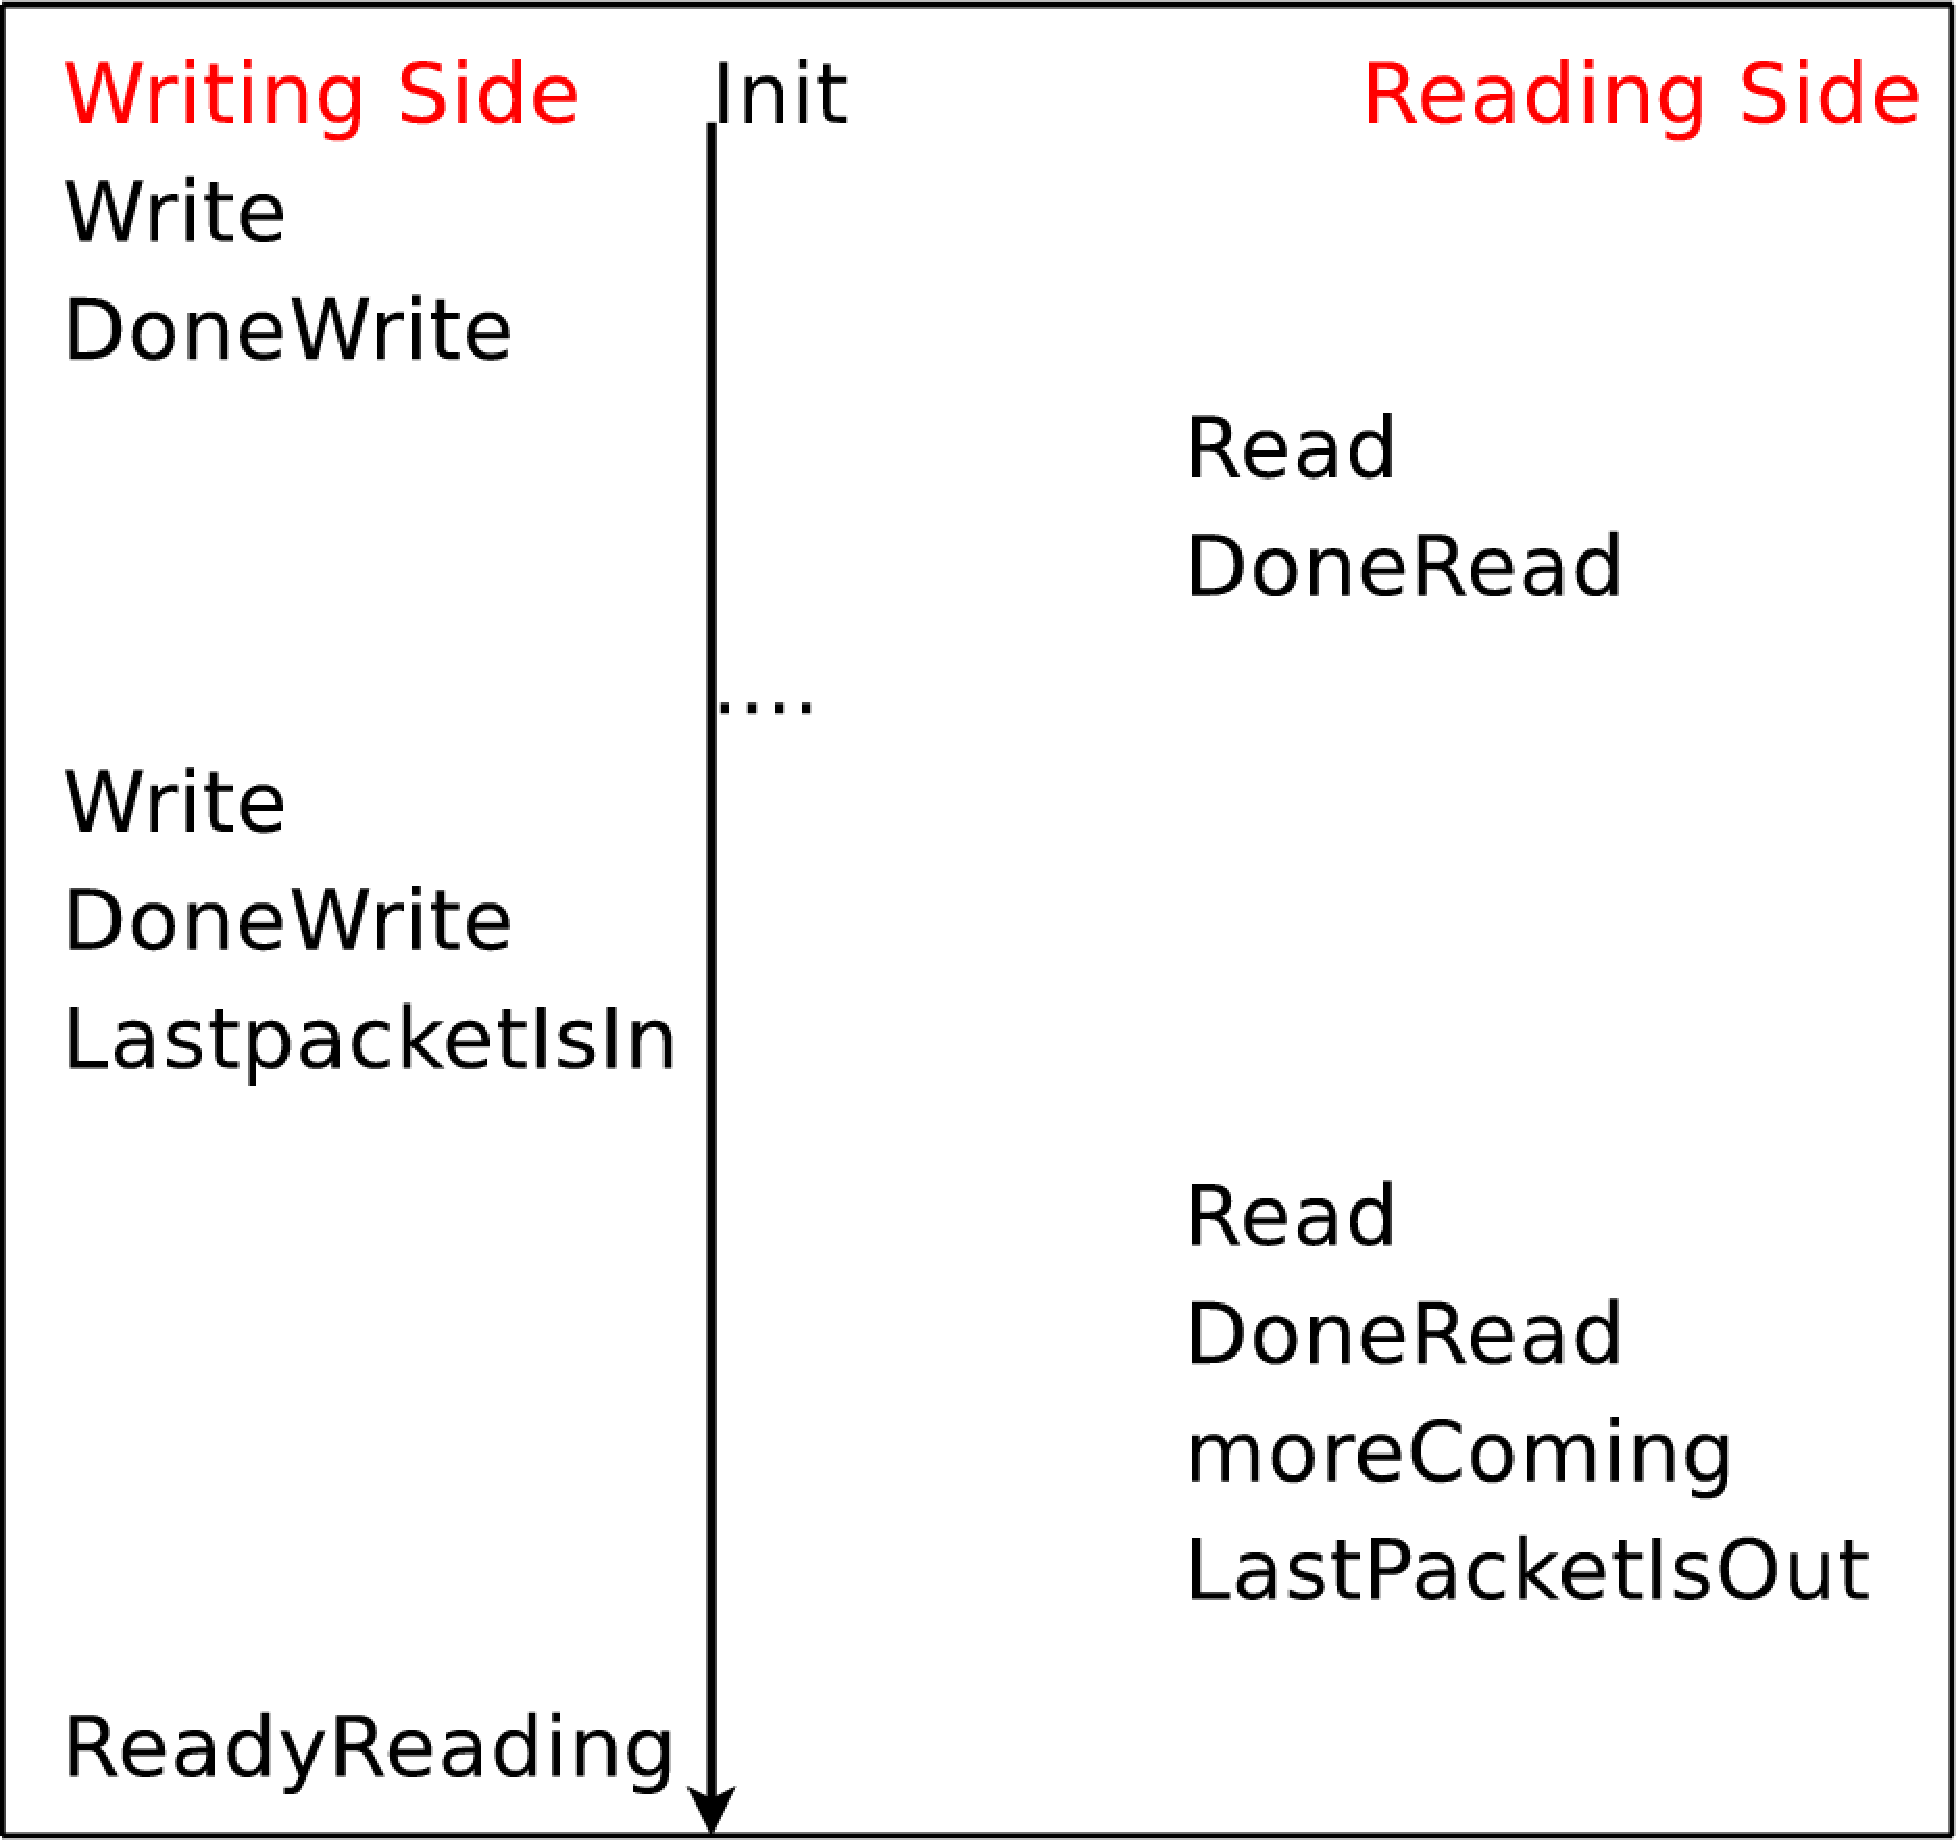
\includegraphics[width=.4\textwidth]{diagrams/order.pdf}
	\caption{Order of operation in a typical setting}
\end{figure}

% void    cb_init(CircularBuffer *cb, euint8* mem, euint32 numsectors, euint32 sectorsize);
% 
% euint8* cb_readPacket(CircularBuffer *cb);
% void    cb_doneReadPacket(CircularBuffer *cb);
% void cb_cancelReadPacket(CircularBuffer *cb);
% euint8* cb_writePacket(CircularBuffer *cb);
% void    cb_doneWritePacket(CircularBuffer *cb);
% void cb_cancelWritePacket(CircularBuffer *cb);
% 
% void    cb_lastPacketIsIn(CircularBuffer *cb);
% euint8  cb_moreComing(CircularBuffer *cb);
% void    cb_lastPacketIsOut(CircularBuffer *cb);
% euint8  cb_readyReading(CircularBuffer *cb);

\end{document}